\chapter{需求对话识别数据集构建与模型实现}

对于模型构建方面,我们使用AllenNLP\footnote{https://allennlp.org/},一个基于PyTorch\footnote{https://pytorch.org/}构建的开源NLP库,来实现我们提出的FRMiner。
\section{数据爬取}
我们的数据是通过Scrapy \footnote{https://scrapy.org/}爬取的。Scrapy是用Python实现的一个为了爬取网站数据、提取结构性数据而编写的应用框架。Scrapy常应用在包括数据挖掘,信息处理或存储历史数据等一系列的程序中。通常我们可以很简单的通过Scrapy框架实现一个爬虫,抓取指定网站的内容或图片。如图\ref{fig:scrapy}所示,Scrapy主要有以下组件构成:Scrapy Engine,Scheduler,Downloader,Spiders,Item Pipeline,Downloader middlewares,Spider middlewares。
\begin{figure}[htbp]
    \centering
    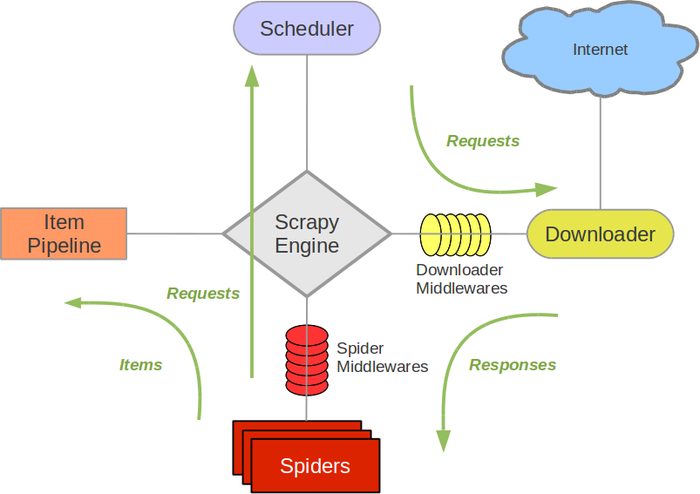
\includegraphics[width=0.6\textwidth]{Img/scrapy.png}
    \bicaption{Scrapy架构图}{The architecture of Scrapy}
    \label{fig:scrapy}
\end{figure}
Scrapy中需要用户自定义的一个核心的组件为Item,其存储了待爬取的对象结构信息。图\ref{fig:echelog}所示为AngularJS项目的IRC记录的格式与内容。
\begin{figure}[htbp]
    \centering
    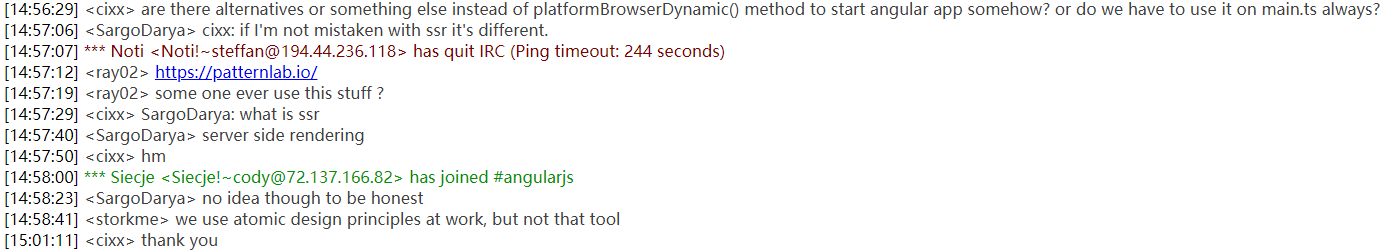
\includegraphics[width=\textwidth]{Img/echelog.png}
    \bicaption{AngularJS项目IRC记录样例。}{An example of AngularJS IRC channel.}
    \label{fig:echelog}
\end{figure}
因此针对IRC数据,我们爬取的Item对象的主要结构信息有:Timestamp,UserName和Message。
爬取的对象主要三个开源项目:AngularJS \footnote{https://angularjs.org/},Bootstrap  \footnote{https://getbootstrap.com/}和 Chromium \footnote{https://www.chromium.org/}. 我们选取这三个项目主要有以下几个原因:首先,它们是最近非常活跃的项目;另外这些项目中存在着较大的开源社区;这些项目中的开发者也非常活跃地使用在线聊天进行分享观点、有趣的见解以及讨论哪些特征需要在以后进行实现。例如,在过去的三年里,AngularJS社区里每周平均有2,823条对话。另外,这些历史对话在IRC Archive网站\footnote{https://echelog.com/}中进行存档并允许开放访问,其为我们的工作提供了丰富的语料资源。

\section{对话预处理}
我们首先对爬取到的文本中的非ASCII字符如Emojis等转换成ASCII字符串。由于一些低频的Tokens,如URL、邮件地址、代码片段、HTML标签、版本号等对最后的分类结果不会产生帮助,因此我们对其分别使用\textit{<URL>,<EMAIL>,<HTML>,<CODE>,<ID>}等特殊Tokens进行替换。然后,我们使用Spacy \footnote{https://spacy.io/}把句子进行分句、分词。为了减少词语形态学的影响,我们使用Spacy对单词进行词干还原和小写转换。

对对话数据进行基本的预处理之后,我们使用JK Kummerfeld等人\cite{kummerfeld2018large}发布的使用其标注数据上训练的模型对我们爬取的数据进行对话解耦,在经过人工审核之后,解耦之后的对话质量、可读性以及解耦的准确性较高,达到了可用标准。
对对话进行解耦之后,我们获取了大量的聊天对话。为了接下来进行数据标注的可行性,并且保证整个对话数据集的整体分布,我们从这三个项目中分别随机采样了400个对话。然后,我们从中过滤掉以下一些质量较低的对话:
\begin{enumerate}
    \item 使用非英语文本的对话
    \item 包含大量代码和Stack Traces信息的对话
    \item 存在大量拼写错误和语法错误的低质量对话
    \item 包含Channel Robots的对话。
\end{enumerate}

\section{数据标注}
标注的对话可以用作我们评估效果的数据集。为了保证标注结果的正确性,我们建立了一个标注小组,由两名资深研究人员和四名博士生组成。他们都具有较高的英语水平,并且在软件开发方面做过深入的研究工作,或者为开源项目做出了积极的贡献。我们将团队分为两组。每个小组由一名负责人(高级研究员)和两名成员组成。每个负责人培训了相应成员如何标注标签并为成员提供咨询。成员对标签的标注结果由负责人进行审查,而每组负责人的结果由其他负责人进行审查。仅当对话在各小组之间的标注达成完全一致时,我们才接受此对话并将对话以及其标签加入到我们的数据集中。而当对话被标注为不同的标记结果时,我们将与所有六个人进行讨论,然后通过投票决定最终标签。表\ref{tab:dataset}为爬取到的所有数据集和我们标注的数据集的统计情况。我们总共从三个开源项目中收集了65,428个对话,并花了720人/小时的时间来标注1,035个对话(总体数据集的1.6%)。

\begin{table}[htbp]
\bicaption{标注对话的统计详情}{The statistic of labeled dialogues}
    \label{tab:dataset}
    \centering
    \footnotesize% fontsize
    \setlength{\tabcolsep}{4pt}% column separation
    \renewcommand{\arraystretch}{1.2}%row space 
\begin{tabular}{|c|c|c|c|c|c|c|}
\hline
\multirow{}{}{} & \multicolumn{3}{c|}{全部聊天记录数据}    & \multicolumn{3}{c|}{抽取样本} \\ \cline{2-7} 
                  & 时间区间          & 对话数   & 句子数    & 对话数    & 句子数     & 特征请求数  \\ \hline
AngularJS         & 2016.5-2019.4 & 38266 & 406553 & 316    & 9220    & 36     \\ \hline
Bootstrap         & 2014.7-2019.5 & 10358 & 58871  & 379    & 2371    & 76     \\ \hline
Chromium          & 2015.5-2019.7 & 16804 & 118890 & 340    & 4465    & 27     \\ \hline
\multicolumn{2}{|c|}{总计}          & 65428 & 584314 & 1035   & 16056   & 139    \\ \hline
\end{tabular}
\end{table}
\section{孪生网络数据集构建}
不同于传统的文本分类模型,我们在数据集构建阶段需要分别对训练集和测试集进行Pair-Instance数据集构建。因此,我们针对p-FRMiner和FRMiner同时实现Single-Instance和Pair-Instance的数据集构建方法。对于p-FRMiner和FRMiner,我们同时实现两种数据集读取方式:lazy读取和一次性加载内存方式。其中lazy方式每次读取一行,然后构建对应Instance,也可以每次读取并构建一个Batch的Instance,以避免数据集过大不能同时加载到内存导致的程序运行问题。

p-FRMiner实现的Dataset Reader中的Instance包含三个元素:dialog矩阵,矩阵的每一行为一个句子分词后的词序列,句子组成的行序列对应句子在原对话中的序列;pos-tag矩阵,矩阵的每一行为一个句子分词后对应的pos-tag序列,句子组成的行序列对应句子在原对话中的序列,因此,pos-tag矩阵中的每个元素对应dialog矩阵每个元素词的pos-tag;label标签,分别以\textit{feature}和\textit{other}代表\textit{feature dialog}和\textit{non-feature dialog}。

而FRMiner为了组建Pair-Instance,其Dataset Reader的实现方式与p-FRMiner的Dataset Reader有所不同。在构建训练集时,遍历原始Single-Instance数据集,对于一个Dialog Instance—— $Dialog_1$,我们从训练集中同时采样一个正样本,也即label为\textit{feature}的$Dialog\_pos$和一个负样本$Dialog\_neg$,和$Dialog_1$组成两个Pair-Instance,即$<Dialog_1,Dialog\_pos>$和$<Dialog_1,Dialog\_neg>$,为了对数据集进行进一步增强以及减少随机采样带来的误差,我们对以上流程在整个数据集上及进行$iter\_num$次。





\section{分层上下文敏感对话模型构建}

\section{孪生网络对话分类模型构建}

\section{训练及模型调参}

对于超参数,我们使用Grid Search\cite{Bergstra2012Random}作为参数选择方法以获得最佳效果。pos-tag向量的维度为50,与单词向量相同。然后,我们可以使用$s=[w_1,w_2\dots w_n]$ 作为句子的表示形式,其中$w_i=[we_i\oplus pos_i]$。为了获得由不同尺度的局部信息组合而成的更充分的语义信息,我们对句子应用具有不同大小的多个卷积核。我们设置了4种不同的卷积核大小,分别是2、3、4、5,每类卷积核有25个。BiLSTM的输出尺寸为300(每个方向150)。我们使用线性层作为相似性度量层,然后将300维向量映射到两个值,这些值表示两个类别的概率得分。由于该任务可以视为分类问题,因此我们将交叉熵用作损失函数。

此外,为避免过拟合问题,我们以0.1的dropout rate对输入向量进行Dropout \cite{srivastava2014dropout},这意味着将随机屏蔽10%的神经元以减少每次批量训练中需要训练的参数。我们还使用了Early Stopping\cite{prechelt1998early}的策略,如果测试数据集的效果在10个Epoch内未提升,则训练过程将停止。
\section{本章小结}